\documentclass[11pt,oneside]{article}
\input{../../../Header/packages.sty}
\input{../../../Header/styleScript.sty}
\input{../../../Header/headerScript.sty}
\input{../../../Header/mathexpressions.sty}


\newcommand{\Skriptname}{Lektion: Der Kathetensatz}
\newcommand{\Autor}{Jonas Guler (Gu)}
\newcommand{\version}{\textit{v}1.0}

\begin{document}
\thispagestyle{plain}
\begin{center}
	{\Huge\textbf{Der Kathetensatz}}\\[3mm]
	{\large Sätze im rechtwinkligen Dreieck -- Aufbau auf dem Satz des Pythagoras}\\[2mm]
	{\normalsize Name: \gap{6}\hspace{1cm} Datum: \gap{3}}
\end{center}
\vspace{2mm}
In dieser Lektion verwenden wir die Bezeichnungen aus dem Skript: Im rechtwinkligen Dreieck $\triangle ABC$ mit $\gamma=90^\circ$ ist $c$ die Hypotenuse, $a$ und $b$ sind die Katheten. Die Höhe $h_c$ teilt die Hypotenuse in die Hypotenusenabschnitte $p$ (bei $A$, also an der Kathete $b$) und $q$ (bei $B$, also an der Kathete $a$).
\begin{center}
	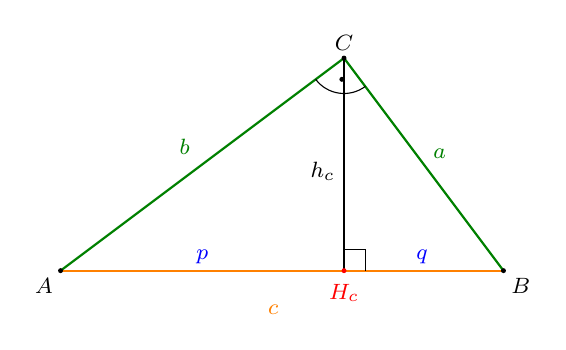
\begin{tikzpicture}[x=1cm, y=1cm, >=latex, font=\footnotesize, scale=0.9]
		\coordinate (A) at (0,0);
		\coordinate (B) at (6.25,0);
		\coordinate (C) at (4,3);
		\coordinate (H) at (4,0);
		\draw[color=orange, line width=0.8pt] (A) -- (B);
		\draw[color=green!50!black, line width=0.8pt] (B) -- (C) -- (A);
		\draw (C) -- (H);
		% rechte Winkel
		\draw [shift={(4,3)}] (-143.13:0.5) arc (-143.13:-53.13:0.5);
		\fill (3.97,2.7) circle (1pt);
		\draw (4.3,0) -- (4.3,0.3) -- (4,0.3);
		\begin{scriptsize}
			\fill (A) circle (1pt) node[below left] {$A$};
			\fill (B) circle (1pt) node[below right] {$B$};
			\fill (C) circle (1pt) node[above] {$C$};
			\fill[red] (H) circle (1pt) node[below=2pt, red] {$H_c$};
			\draw[color=orange] (3,-0.55) node {$c$};
			\draw[color=green!50!black] (5.35,1.65) node {$a$};
			\draw[color=green!50!black] (1.75,1.75) node {$b$};
			\draw (3.7,1.4) node {$h_c$};
			\draw[color=blue] (2,0.2) node {$p$};
			\draw[color=blue] (5.1,0.2) node {$q$};
		\end{scriptsize}
	\end{tikzpicture}
\end{center}

%############################################################################################
\section{Einstieg: Katheten und Hypotenusenabschnitte}
\begin{aufgabe}[Entdeckungsaufgabe, Partnerarbeit] % Idee: Geometrie 1 Aufgaben (Niederberger) Kap. 5.2 Nr. 44
	\textbf{Teil A: Rechnen mit Pythagoras.} Gegeben ist ein rechtwinkliges Dreieck mit $\gamma=90^\circ$, $a=15$ cm und $b=20$ cm.
	\begin{enumerate}[label=\alph*)]
		\item Berechne die Länge der Hypotenuse $c$.
		\item Berechne die Höhe $h_c$. \textit{Tipp: Berechne den Flächeninhalt des Dreiecks auf zwei verschiedene Arten.}
		\item Berechne die beiden Hypotenusenabschnitte $p$ und $q$. \textit{Tipp: Die Höhe $h_c$ zerlegt das Dreieck in zwei rechtwinklige Teildreiecke.}
	\end{enumerate}
	\karos{7}
	\begin{enumerate}[label=\alph*), resume]
		\item Ergänze die Tabelle. Die Werte für das zweite Dreieck ($a=6$ cm, $b=8$ cm) sind teilweise bereits berechnet.
	\end{enumerate}
	\begin{center}
		\renewcommand{\arraystretch}{1.8}
		\begin{tabular}{|*{10}{>{\centering\arraybackslash}p{8.5mm}|}}\hline
			$a$ & $b$ & $c$ & $h_c$ & $p$ & $q$ & $a^2$ & $c\cdot q$ & $b^2$ & $c\cdot p$ \\\hline\hline
			$15$ & $20$ & & & & & & & & \\\hline
			$6$ & $8$ & $10$ & $4.8$ & $6.4$ & $3.6$ & & & & \\\hline
		\end{tabular}
	\end{center}
	\begin{enumerate}[label=\alph*), resume]
		\item Was fällt dir auf? Formuliere eine Vermutung in Worten und als Formel.
	\end{enumerate}
	\karos{2.5}\\[3mm]
	\textbf{Teil B (für Schnelle): Lässt sich die Vermutung beweisen?} Betrachte ein allgemeines rechtwinkliges Dreieck wie in der Figur oben.
	\begin{enumerate}[label=\alph*), resume]
		\item Wende den Satz des Pythagoras dreimal an: im Teildreieck $\triangle H_cBC$, im Teildreieck $\triangle AH_cC$ und im ganzen Dreieck $\triangle ABC$ (mit $c=p+q$). Notiere die drei Gleichungen.
		\item Subtrahiere die zweite Gleichung von der ersten und addiere das Resultat zur dritten. Was erhältst du?
	\end{enumerate}
	\karos{6}
\end{aufgabe}

\newpage
%############################################################################################
\section{Der Kathetensatz}
Die Vermutung aus der Einstiegsaufgabe gilt in jedem rechtwinkligen Dreieck. Geometrisch betrachtet vergleicht sie die Fläche eines Quadrates mit der Fläche eines Rechtecks.
\begin{satz}[Kathetensatz oder Satz des Euklid]
	\begin{minipage}{0.5\linewidth}
		In einem rechtwinkligen Dreieck ist das Quadrat über einer Kathete flächengleich wie das Rechteck aus der Hypotenuse und dem \textbf{an dieser Kathete anliegenden} Hypotenusenabschnitt:
		\[a^2=c\cdot q \qquad\text{und}\qquad b^2=c\cdot p.\]
	\end{minipage}
	\hfill
	\begin{minipage}{0.45\linewidth}
		\centering
		\begin{tikzpicture}[x=1cm, y=1cm, >=latex, font=\footnotesize, scale=0.48]
			% Dreieck: A(0,0), B(5,0), C(3.2,2.4); b=4, a=3, c=5, p=3.2, q=1.8
			\filldraw[fill=myblue, fill opacity=0.25, draw=black] (0,0) -- (3.2,2.4) -- (0.8,5.6) -- (-2.4,3.2) -- cycle;
			\filldraw[fill=orange, fill opacity=0.25, draw=black] (3.2,2.4) -- (5,0) -- (7.4,1.8) -- (5.6,4.2) -- cycle;
			\filldraw[fill=myblue, fill opacity=0.25, draw=black] (0,0) -- (3.2,0) -- (3.2,-5) -- (0,-5) -- cycle;
			\filldraw[fill=orange, fill opacity=0.25, draw=black] (3.2,0) -- (5,0) -- (5,-5) -- (3.2,-5) -- cycle;
			\draw[line width=1pt] (0,0) -- (5,0) -- (3.2,2.4) -- cycle;
			\draw[dashed] (3.2,2.4) -- (3.2,0);
			\begin{scriptsize}
				\draw (-0.3,-0.1) node[left] {$A$};
				\draw (5.3,-0.1) node[right] {$B$};
				\draw (3.2,2.6) node[above] {$C$};
				\draw (-0.6,2.6) node {$b^2$};
				\draw (5.3,2.1) node {$a^2$};
				\draw (1.6,-2.5) node {$c\cdot p$};
				\draw (4.1,-2.5) node {$c\cdot q$};
				\draw (1.6,0.25) node {$p$};
				\draw (4.1,0.25) node {$q$};
				\draw (5.35,-2.5) node[right] {$c$};
			\end{scriptsize}
		\end{tikzpicture}
	\end{minipage}
\end{satz}
\begin{beweis}
	Mit dem Satz des Pythagoras in den beiden Teildreiecken und im ganzen Dreieck gilt:
	\[\text{(I)}\ a^2=\gap{2.2}, \qquad \text{(II)}\ b^2=\gap{2.2}, \qquad \text{(III)}\ a^2+b^2=(p+q)^2=\gap{2.5}\]
	\karos{3}
\end{beweis}
\textbf{Bemerkungen:}
\begin{itemize}
	\item Umgekehrt folgt aus dem Kathetensatz sofort der Satz des Pythagoras: $a^2+b^2=c\cdot q+c\cdot p=\gap{4}$.\\[2mm] Genau so hat Euklid (ca. 300 v. Chr.) den Satz des Pythagoras in seinen \textit{Elementen} bewiesen.
	\item Mit dem Kathetensatz lassen sich die Hypotenusenabschnitte direkt aus den Seiten berechnen: \[q=\gap{2} \qquad\text{und}\qquad p=\gap{2}.\]
	\item \textbf{Achtung:} Liegt der rechte Winkel nicht bei $C$, so ändern sich die Namen. Merke dir den Satz deshalb in Worten: \textit{Kathete$^2$ = Hypotenuse $\cdot$ anliegender Hypotenusenabschnitt}.
\end{itemize}

\begin{beispiel}
	Im rechtwinkligen Dreieck $\triangle ABC$ mit $\gamma=90^\circ$ sind $a=6$ cm und $c=9$ cm gegeben. Berechne $q$, $p$ und $b$ ohne zuerst $b$ mit Pythagoras zu bestimmen und kontrolliere dein Resultat anschliessend mit dem Satz des Pythagoras.
\end{beispiel}
\karos{4}

%############################################################################################
\section{Übungen}
\setcounter{aufg}{0}
\begin{aufgabe}[Grundaufgaben] % angelehnt an Geometrie 1 Aufgaben Kap. 5.2 Nr. 43, 47 und Geometrie 2 (Niederberger) S. 82 Nr. 4
	Berechne in den rechtwinkligen Dreiecken $\triangle ABC$ mit $\gamma=90^\circ$ (Bezeichnungen wie in der Figur auf Seite 1) die gesuchten Grössen. Mache jeweils eine Skizze.
	\begin{enumcols}[2]
		\item $a=4$ cm, $b=3$ cm. Gesucht: $c,p,q$.
		\item $c=16$ cm, $b=12$ cm. Gesucht: $p,q$.
		\item $p=2$ cm, $q=8$ cm. Gesucht: $a,b$.
		\item $b=10$ cm, $p=8$ cm. Gesucht: $c,q,a$.
		\item $c=13$ cm, $a=5$ cm. Gesucht: $p,q,b$.
		\item $a=\sqrt{12}$ cm, $q=2$ cm. Gesucht: $c,p,b$.
	\end{enumcols}
	\karos{11}
\end{aufgabe}

\begin{aufgabe}[Lot auf die Diagonale] % angelehnt an Geometrie 2 (Niederberger) S. 82 Nr. 5
	Im Rechteck $ABCD$ gilt $\overline{AB}=20$\,cm und $\overline{BC}=15$\,cm. Das Lot von $B$ auf die Diagonale $AC$ hat den Fusspunkt $E$. Mache eine Skizze und berechne die Längen $\overline{AE}$, $\overline{CE}$ und $\overline{BE}$.\par
	\karos{6}
\end{aufgabe}

\begin{aufgabe}[Kathete und Abschnitt]
	In einem rechtwinkligen Dreieck mit $\gamma=90^\circ$ misst die Hypotenuse $c=10$ cm. Die Kathete $a$ ist doppelt so lang wie der Hypotenusenabschnitt $q$. Berechne $a$, $q$, $p$ und $b$.\par
	\karos{5}
\end{aufgabe}

\begin{aufgabe}[Ein Rechteck wird zum Quadrat] % angelehnt an Geometrie 2 (Niederberger) S. 81/82 Nr. 1
	Mit dem Kathetensatz lässt sich ein Rechteck in ein flächengleiches Quadrat verwandeln. Gegeben ist ein Rechteck mit den Seitenlängen $4.5$ cm und $2.5$ cm.
	\begin{enumerate}[label=\alph*)]
		\item Zeichne eine Strecke $\overline{AB}$ der Länge $c=4.5$ cm und trage von $B$ aus die Länge $q=2.5$ cm auf $\overline{AB}$ ab. Den so erhaltenen Punkt nennst du $H$.
		\item Errichte in $H$ die Senkrechte zu $AB$ und zeichne den Thaleskreis über $\overline{AB}$. Der Schnittpunkt der beiden ist $C$.
		\item Begründe mit dem Kathetensatz, weshalb das Quadrat über $\overline{BC}$ denselben Flächeninhalt hat wie das Rechteck. Zeichne das Quadrat.
		\item Kontrolliere: Miss $\overline{BC}$ und vergleiche mit dem berechneten Wert.
	\end{enumerate}
	\karos{8}
\end{aufgabe}

\begin{aufgabe}[$\bigstar$ Knobelaufgabe: Raumdiagonale] % Geometrie 2 (Niederberger) S. 82 Nr. 7
	Der Quader $ABCDEFGH$ hat die Kantenlängen $\overline{AB}=8$ cm, $\overline{BC}=6$ cm und $\overline{AE}=7.5$ cm. Der Fusspunkt des Lotes von $D$ auf die Raumdiagonale $BH$ heisst $P$. Berechne das Verhältnis $\overline{BP}:\overline{HP}$.\\
	\textit{Tipp: Suche ein rechtwinkliges Dreieck mit Hypotenuse $\overline{BH}$, das den Punkt $D$ enthält.}\par
	\karos{6}
\end{aufgabe}

\end{document}
